%%%%%%%%%%%%%%%%%%%% author.tex %%%%%%%%%%%%%%%%%%%%%%%%%%%%%%%%%%%
%
%%%%%%%%%%%%%%%% Springer %%%%%%%%%%%%%%%%%%%%%%%%%%%%%%%%%%


%Sections that need work still:
%1. Flesh out the outline
%2. Needs to be filled out some, including citations
%3. Done
%4. Done
%5. Are we worried about grayscale?
%   - Otherwise, seems done
%6. Mostly done. There's one unwritten paragraph at the end that either needs to be written or removed. The rest is solid, but wouldn't hurt to go over it again.
%7. Flesh out the outline


\title*{Lexicase selection for program synthesis: a diversity analysis}
\titlerunning{Lexicase selection for program synthesis: a diversity analysis}
% Use \titlerunning{Short Title} for an abbreviated version of
% your contribution title if the original one is too long
\author{Thomas Helmuth, Nicholas Freitag McPhee, Lee Spector}
% Use \authorrunning{Short Title} for an abbreviated version of
% your contribution title if the original one is too long
\institute{Thomas Helmuth \at Computer Science, University of Massachusetts, Amherst, MA USA
\and Nicholas Freitag McPhee \at Division of Science and Mathematics, University of Minnesota, Morris, MN USA
\and Lee Spector \at Cognitive Science, Hampshire College, Amherst, MA USA}

\maketitle

\abstract{Lexicase selection is a selection method for  evolutionary computation in which individuals are selected by filtering the population by performance on individual fitness cases, considered in random order. Lexicase selection, when used as the parent selection method in genetic programming, has been shown to provide significant improvements in terms of problem-solving power. In this chapter we investigate the reasons for the success of lexicase selection, focusing in particular on the ways in which lexicase selection seems to help maintain population diversity. We present data from eight program synthesis problems and compare lexicase selection, in terms of problem solving power and diversity, to tournament selection and selection based on implicit fitness sharing. We conclude that lexicase selection does indeed produce more diverse populations, and that this helps to explain the utility of lexicase selection for program synthesis.}

\begin{keywords}
Lexicase selection, diversity.
\end{keywords}
\index{keywords to your chapter}
\index{these words should also be indexed}

\section{Introduction} \label{intro}

Lexicase selection is a recent selection method for  evolutionary computation in which individuals are selected by 
filtering the population by performance on individual fitness cases, considered in random order. Lexicase 
selection, when used as the parent selection method in genetic programming, has been shown to provide 
significant improvements in terms of problem-solving power (\cite{Helmuth:2015:ieeeTEC,Helmuth:2015:GECCO}). 
In this chapter we investigate the reasons for the success of lexicase selection, focusing in particular on the 
ways in which lexicase selection seems to help maintain population diversity. We present data from eight 
program synthesis problems and compare lexicase selection, in terms of problem solving power and diversity, 
to tournament selection and selection based on implicit fitness sharing (IFS).

We use two measures of popuation diversity to explore the impact of these selection mechanisms: 
Error diversity and cluster counts. We find that lexicase runs have consistently 
higher error diversity than tournament selection and IFS across all generations and all problems; the cluster 
count values for lexicase are also generally higher, but those results are less consistent. Based on these results 
we conclude that lexicase selection does indeed produce more diverse populations, and that this helps to explain 
the utility of lexicase selection for program synthesis.

\section{Lexicase selection}

\marginpar{(NEEDS WORK: include description, brief account of prior work, and important properties)}
	
Pseudocode for the lexicase selection algorithm is outlined in 
Algorithm~\ref{alg:lexicase}. In each parent selection event, the lexicase selection algorithm 
first randomly orders the test cases. It then eliminates any individuals in the population 
that do not have the best performance on the first test case. 
Assuming that more than one individual remains, it then loops, eliminating any individuals from 
the remaining candidates that do not have the best performance on the second test case. This 
process continues until only one individual remains and is selected, or until all test cases 
have been used, in which case it randomly selects one of the remaining individuals.

\begin{algorithm}[tb]
	\begin{algorithmic}
		\STATE \texttt{candidates} $:=$ the entire population
		\STATE \texttt{cases} $:=$ list of all the test cases in a random order
		\WHILE{$|\texttt{candidates}|>1$ \AND $|\texttt{cases}|>0$}
			\STATE \texttt{current}, \texttt{cases} := $\textrm{first}(\texttt{cases})$, $\textrm{rest}(\texttt{cases})$
			\STATE \texttt{best\_performance} $:= \min \{ \textrm{perf}(i, \texttt{current}) \;|\; i \in \texttt{candidates} \}$
			\STATE \texttt{candidates} := $\{ i \;|\; i \in \texttt{candidates} \;\land\; \textrm{perf}(i, \texttt{current}) = \texttt{best\_performance}\}$
		\ENDWHILE
		\RETURN random individual from \texttt{candidates}
	\end{algorithmic}
	\caption{Psuedocode for the lexicase selection algorithm. The use of $\min$ when computing 
		\texttt{best\_performance} assumes that the goal is to minimize on each test case, which
		is true in the work presented here, where the goal for all test cases is to minimize error.
		This can be easily generalized to other settings.}
	\label{alg:lexicase}
\end{algorithm}

The central properties of lexicase selection are that (a) it doesn't combine all the errors into a single
fitness value and (b) because of the random ordering of test cases, every test case is likely to be
most important (first to be considered) at least occasionally. With a population of 1,000 individuals
and a problem with 200 test cases, for example, we would expect each test case to be first several
times in each generation. The hope, then, is that this ensures some diversity in the population, with
different (groups of) individuals being rewarded for their ability to perform well on different test
cases.


\section{Explorations of Population Dynamics}
\label{sec:exploration}


The key goal of this paper is to try to better understand why lexicase outperforms tournament selection
and IFS on a variety of problems. One hypothesis is that lexicase helps maintain population diversity
by randomizing the priority of test cases at each selection event, ensuring for example that each test 
case is the most important several times each generation. Here we test this hypothesis by measuring 
diversity in two different ways, error diversity and population clustering, and compare the results 
for lexicase, tournament selection, and IFS.

\subsection{Error Diversity}
\label{sec:errorDiversityDef}

\textit{Error diversity} measures the semantic diversity of a population as the percent of distinct error vectors in the population. When evaluating a program, it is tested on a set of test cases composed of input/output pairs. Then, one or more error functions are applied to the desired output and the program's output, creating an error vector for each individual.

Error diversity is similar to \textit{behavioral diversity}, which calculates the percent of distinct behavior vectors in the population \citep{Jackson:2010:PPSN}. Here, the behavior of a program is the vector of outputs a program produces when run on the vector of inputs. Error diversity for a population will be less than or equal to its behavioral diversity, since two different behavior vectors may produce the same error vector, but two different error vectors must come from different behavior vectors.

\cite{Helmuth:2015:ieeeTEC} showed that in sets of runs in which lexicase selection achieved higher success rates, 
it also maintained higher population diversity. Here, we  explore whether similar 
effects are seen in error diversity across other problems.

\subsection{Population Clustering}
\label{sec:clusterCountDef}

One hypothesis we have developed as to why lexicase selection has led to improved performance compared to tournament selection and IFS is that it enables a population to develop groups of individuals that evolve side-by-side, similar to more explicit niching methods such as island models. These groups would specialize in solving specific subsets of the training set. We expect that evolution may sometimes progress when two individuals from separate groups mate, creating a child that combines the abilities of each parent, creating a larger group that combines the parents' specializations. If crossover continues combining groups throughout evolution, we hope that eventually an individual will be created that combines the requirements of all of the training cases, solving the problem.

We would like to explore the effects of different parent selection methods on the development of these clusters of individuals that perform similarly across the test cases. We expect that using lexicase selection will result in larger numbers of clusters than tournament selection or IFS, since it emphasizes the selection of individuals that specialize on specific test cases rather than performing adequately across all test cases.

To examine this idea of clusters within a single population, we must be able to measure the clustering of a population with respect to the training cases. Our approach here is to use a clustering algorithm to find the number of clusters that exist in a population, plotting a measurement of the clustering at each generation. We base the clustering of the population on the individuals' error vectors across the training cases. \cite{Krawiec:2015:EuroGP} use a similar approach, except that they cluster the test cases into some number of search objectives based on the individuals, where we cluster the individuals into groups based on the test cases.


Since we are primarily interested in whether an individual performs at least as well as every other 
individual in the population, we convert the error vectors into binary ``elitized'' error vectors 
that indicate whether an individual achieved the best error on each test case in that generation. 
More formally, if each individual $j$ in the population $P$ has error vector $error_j$ containing error values on the test cases $T$, then the elitized error vector for individual $i$ is defined by
\[
elitized_i[t] =
\begin{cases}
    0,         & \text{if } error_i[t] = \min\limits_{j \in P} (error_j[t])  \\
    1,         & \text{otherwise}
\end{cases}
\]
for $t \in T$.
By elitizing the error vectors, we can ignore the differences between individuals that perform poorly on cases in different 
ways, and concentrate on how individuals cluster based on the cases on which they perform well.

In this work we use agglomerative clustering to count how many clusters there are in the population 
at each generation. Agglomerative clustering creates 
a hierarchical clustering model by first placing each individual into its own cluster. It then 
iteratively combines the two closest clusters into a single cluster, until all clusters have been 
combined into a single cluster. This single cluster includes the distance between each pair of clusters 
that were combined into a larger cluster. We can break the single cluster into smaller clusters by
``cutting'' the merge between any two clusters whose distance exceeds some threshold.
%\marginpar{Should we include a dendogram and talk about the cutting in terms of levels in the diagram?}
% TMH: I don't think we really have room for one :(

Since we are using binary error vectors, we can use the 
Manhattan distance as our distance metric, which makes the distance between two error vectors
a count of how many test cases on which those two individuals have different ``eliteness'' 
results.\footnote{We used the \texttt{agnes} \citep{cluster} implementation of 
	agglomerative clustering in R \citep{R}, using the \texttt{average} linkage when 
	combining clusters.} 
We chose to count the number of clusters that differed on at least 10\% of the training cases; 
for example, if a problem has 200 training cases, we counted the number of clusters that differed 
in binary elitness on at least 20 training cases. While this distance is somewhat arbitrary, 
it gives a reasonable and consistent estimate of how many groups of individuals are doing 
significantly different things in a given generation.

\section{Experimental setup}
\label{sec:setup}

To better understand the impact of lexicase selection on population diversity, we collected data
from 100 runs each of 8 different problems described in \cite{Helmuth:2015:GECCO}, all of which are
basic programming problems taken from introductory programming texts. Table~\ref{tab:problems} lists
the problems, a brief description, and the length of the error vectors\footnote{For some of these problems, multiple error functions are used for a run of a program on a single test case.}; other details of the runs can be
found in \cite{Helmuth:2015:GECCO}. In Table~\ref{tab:successCounts} we've also provided the number 
of successes, i.e., runs where an program was evolved with total error of 0 across all the test cases, as well as generalizing to an unseen test set.
Success rates aren't the focus of this paper, but those numbers give a sense of the relative
difficulty of the problems and illustrate the substantial improvements that lexicase selection
provides over both tournament selection and IFS.

\begin{table}
\centering
	\caption{Short descriptions of the 8 test problems used here, along with the number of errors in each error vector. See \cite{Helmuth:2015:GECCO} for more details on each problem.}
	\label{tab:problems}
	\begin{tabular}{lp{6.5cm}r}
		Problem name \quad & Description \quad & \# errors \\
		\hline
		Replace Space With Newline & Print the input string, replacing spaces with newlines. Also, return the number of non-whitespace characters. & 200 \\
		Syllables & Count the number of occurrences of vowels (a, e, i, o, u, y) in the given string and print that number as \texttt{X} in \texttt{The number of syllables is X}. & 200 \\
		String Lengths Backwards & Given a vector of strings, print the length of each string in reverse order (starting with last and ending with first). & 100 \\
		Negative To Zero & Given a vector of integers, return the vector where all negative integers have been replaced by 0. & 200 \\
		Double Letters & Given a string, print the string, doubling every letter character, and tripling every exclamation point. All other non-alphabetic and non-exclamation characters should be printed a single time each. & 100 \\
		Scrabble Score & Given a string of visible ASCII characters, return the Scrabble score for that string. & 200 \\
		Checksum & Given a string, compute the integer ASCII values of the characters in the string, sum them, take the sum modulo 64, add the integer value of the space character, and then convert that integer back into its corresponding character (the checksum character). The program must print \texttt{Check sum is X}, where \texttt{X} is replaced by the correct checksum character. & 200 \\
		Count Odds & Return the number of integers in a given vector that are odd. & 200
	\end{tabular}
\end{table}

\begin{table}
\centering
	\caption{Number of successes (out of 100 runs) for each of the 8 test problems used here for each
		tested selection mechanism. These numbers are similar but not identical to those reported in 
		\cite{Helmuth:2015:GECCO} because new runs were performed for this paper.}
	\label{tab:successCounts}
	\begin{tabular}{lrrr}
		Problem name \quad & Lexicase \quad & Tournament \quad & IFS \\
		\hline
		Replace Space With Newline & 55 & 13 & 17 \\
		Syllables & 22 & 1 & 2 \\
		String Lengths Backwards & 75 & 19 & 10 \\
		Negative To Zero & 57 & 15 & 7 \\
		Double Letters & 5 & 0 & 0 \\
		Scrabble Score & 0 & 0 & 0 \\
		Checksum & 0 & 0 & 0 \\
		Count Odds & 3 & 0 & 0 \\
	\end{tabular}
\end{table}

We used the Clojush implementation\footnote{\url{https://github.com/lspector/Clojush}} 
of the PushGP system \citep{spector:2002:GPEM, 1068292} for all runs. Each run used a population size of 1,000 
individuals, and runs continued for either 300 generations or a until solution was found, whichever 
came first. 

%For each run we collected vectors of the test case errors for each individual for every
%generation. These were then used to compute the error diversity (see Section~\ref{sec:errorDiversityDef}
%above) and the number of clusters (see Section~\ref{sec:clusterCountDef}).

\section{Results}
\label{sec:results}

In this section we present plots showing error diversity and cluster counts over time for each of
the eight test problems. Below each plot is a smaller sub-plot showing the number of successes 
over time for each selection; since runs end when a solution is found, the successes plot gives a
sense of how many runs are still being represented in primary plot at a given number of generations.
In Figure~\ref{rswnDiv}, for example, the number of lexicase successes is nearly 25 by generation
50, and nearly 50 by generation 150. Thus there are slightly more than 75 data points still represented
in the lexicase data at generation 50, but only about 50 data points represented from generations 150
to 300. Each plot includes a line indicating the median error diversity or median cluster count across
whichever of the 100 runs was still running at that generation. We also indicate the 
range from the 25\% percentile to the 75\% percentile with a gray band around the median line; 
unfortunately the tournament and IFS results are often very similar and strongly overlap, making them difficult to differentiate.

In general the error diversity numbers for lexicase are substantially and significantly
higher than those for either tournament selection or IFS, both of which tend to be extremely similar.
The String Lengths Backwards problem was the only problem for which there was any substantial overlap 
between the range of values for lexicase and the other two selection mechanisms (see 
Figure \ref{string-lengths-backwardsDiv}). Typically the lexicase error diversity rises very sharply
in the early generations leveling off somewhere between 0.75 and 1.0, meaning that $3/4$ or
more of the individuals in the lexicase runs have unique error vectors. This is in contrast
to the tournament selection and IFS results, where the median error diversity values rarely rise above
0.5; the two exceptions are on the Scrabble Score and Count Odds problems 
(Figures~\ref{scrabble-scoreDiv} and~\ref{count-oddsDiv}), which neither ever
solved, where the error diversity values approach or exceed 0.75.

The cluster count results are more mixed. Lexicase has clearly higher cluster counts for
half of the problems (Replace Space With Newline, Syllables, Scrabble Score, and Count Odds;
Figures~\ref{rswnClu}, \ref{syllablesClu}, \ref{scrabble-scoreClu} and~\ref{count-oddsClu}).
It also starts with much higher counts on the Double Letters problem (Figure~\ref{double-lettersClu}), 
but those numbers drop again quickly, matching the other two approaches by around generation 100. 
On the Negative To Zero problem (Figure~\ref{negative-to-zeroClu}), the lexicase
cluster counts remain small (about the same as for both tournament selection and IFS) throughout the runs.
Particularly striking are lexicase cluster counts for String Lengths Backwards and Checksum, where the
number of clusters with lexicase are actually lower earlier in the run. The number of clusters with
Checksum remain low throughout (Figure~\ref{checksumClu}), while the number of String Lengths Backwards 
clusters climb up to roughly the same values as tournament selection and IFS by around generation 150 
(Figure~\ref{string-lengths-backwardsClu}).

\begin{figure}[p] %[t] sets the image at the top of the page; t = top, b = bottom, h = here%
%\sidecaption[t]
\centering
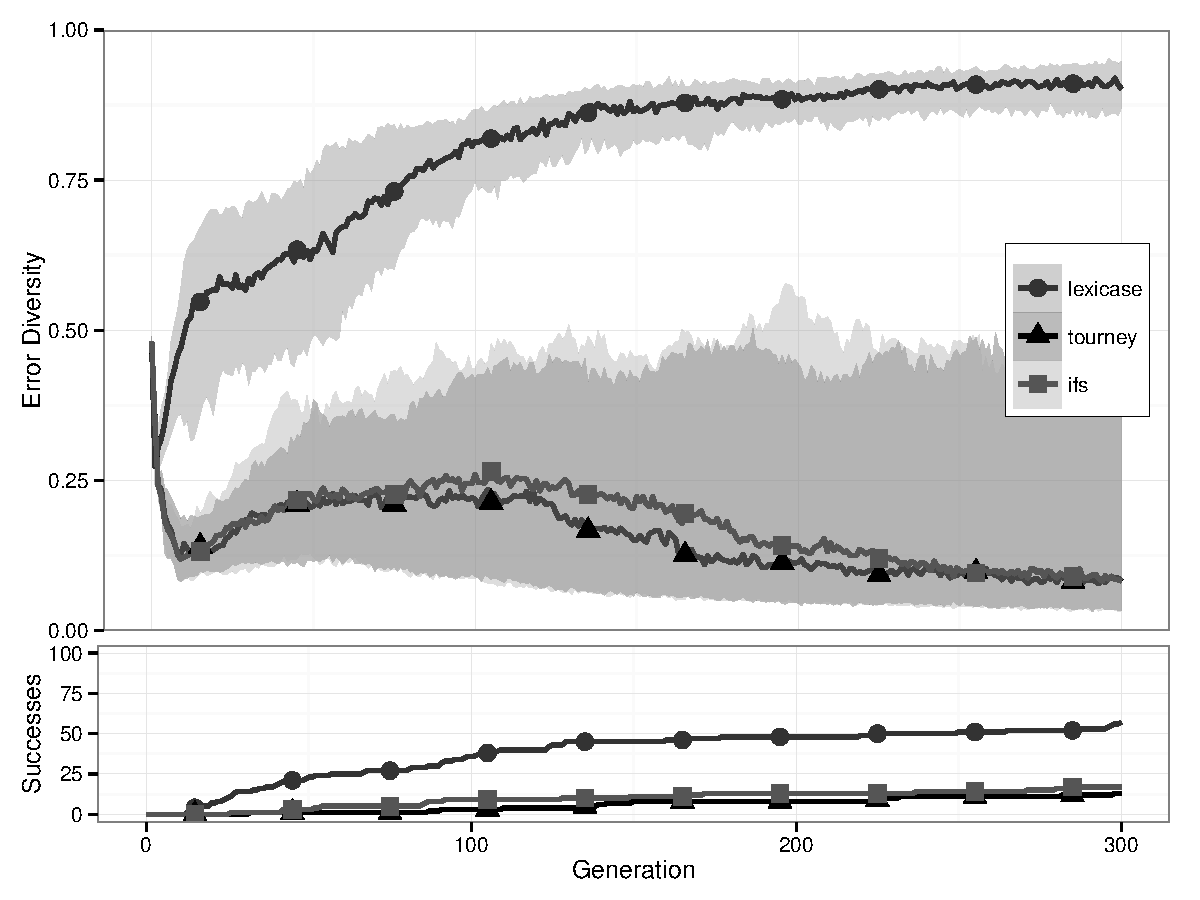
\includegraphics[width=11.5cm]{replace-space-with-newline-diversity.pdf}
\caption{Replace Space With Newline -- error diversity}
\label{rswnDiv}
\end{figure}

\begin{figure}[p] %[t] sets the image at the top of the page; t = top, b = bottom, h = here%
%\sidecaption[t]
\centering
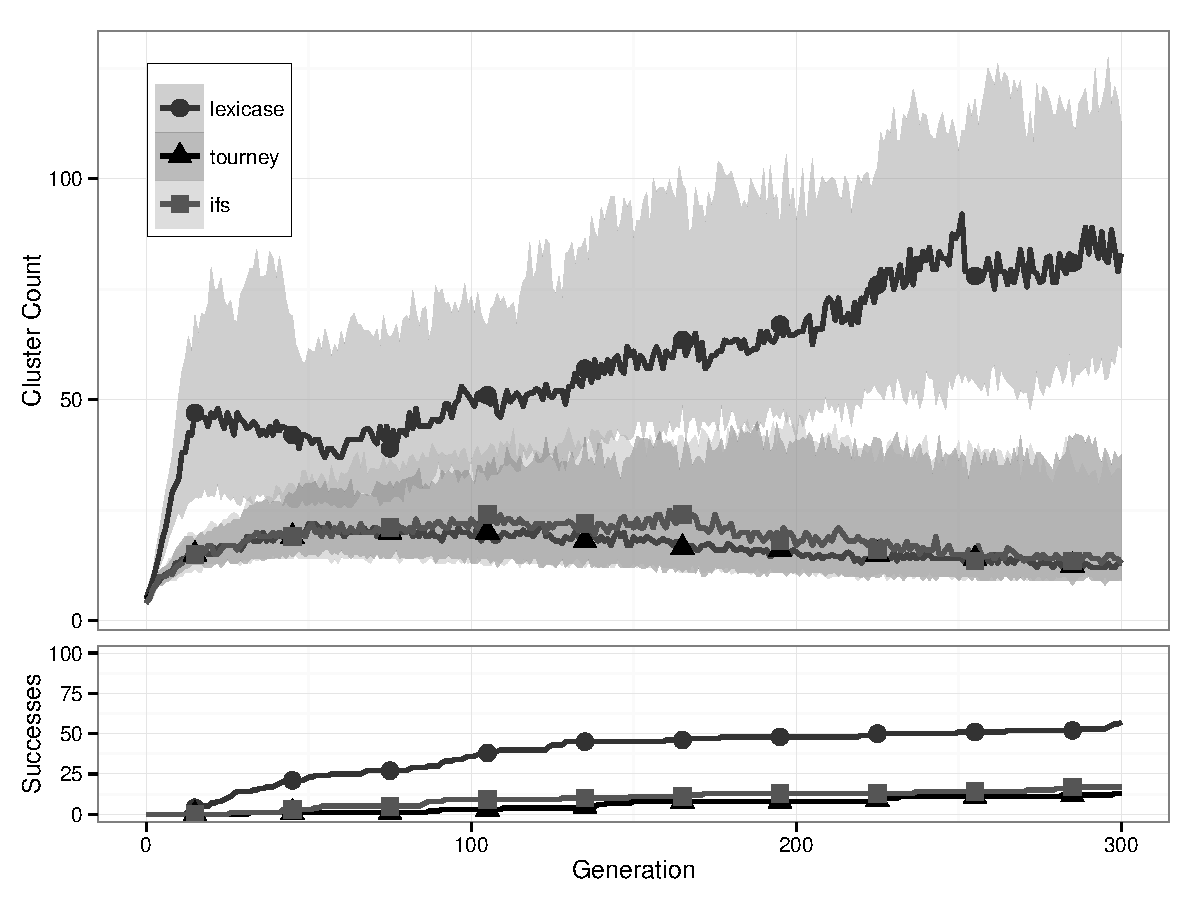
\includegraphics[width=11.5cm]{replace-space-with-newline-cluster.pdf}
\caption{Replace Space With Newline -- cluster counts}
\label{rswnClu}
\end{figure}

\begin{figure}[p] %[t] sets the image at the top of the page; t = top, b = bottom, h = here%
%\sidecaption[t]
\centering
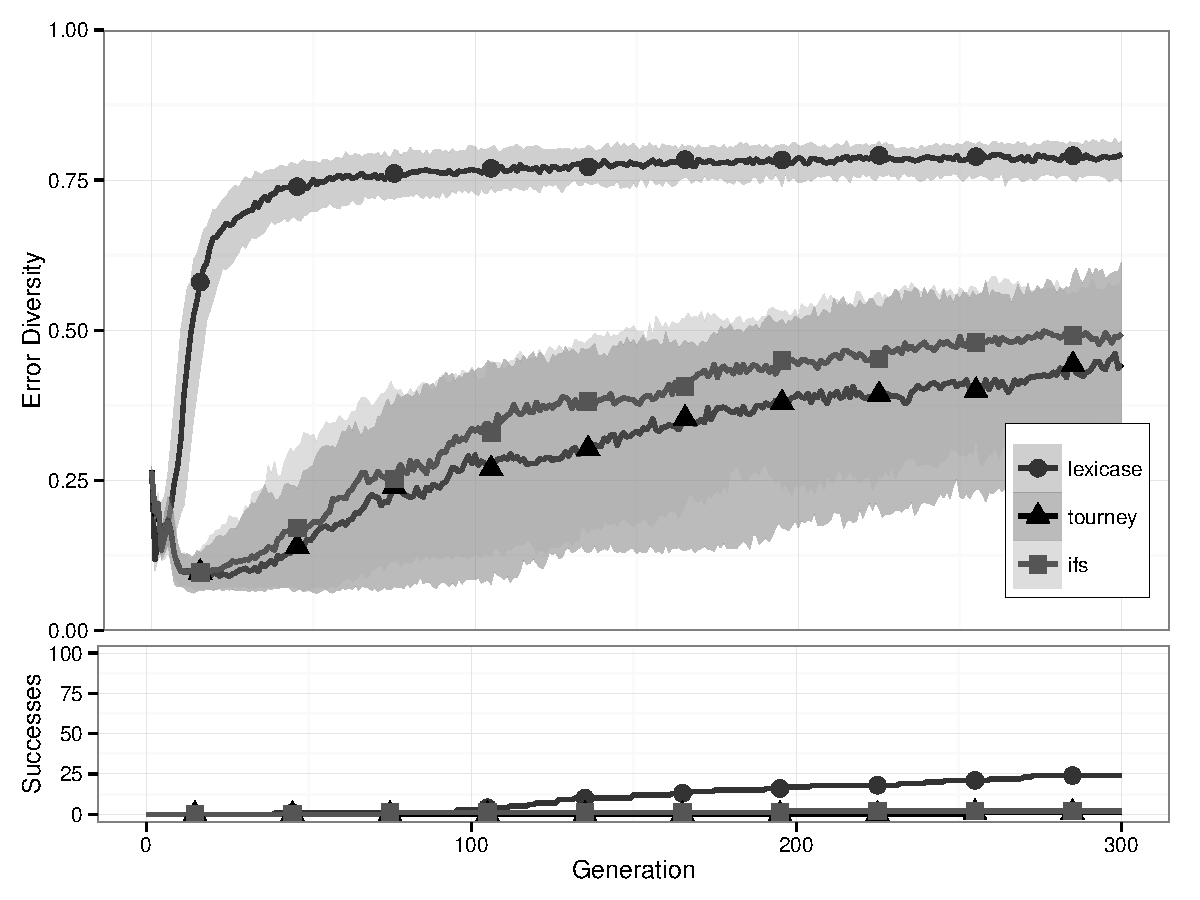
\includegraphics[width=11.5cm]{syllables-diversity.pdf}
\caption{Syllables -- error diversity}
\label{syllablesDiv}
\end{figure}

\begin{figure}[p] %[t] sets the image at the top of the page; t = top, b = bottom, h = here%
%\sidecaption[t]
\centering
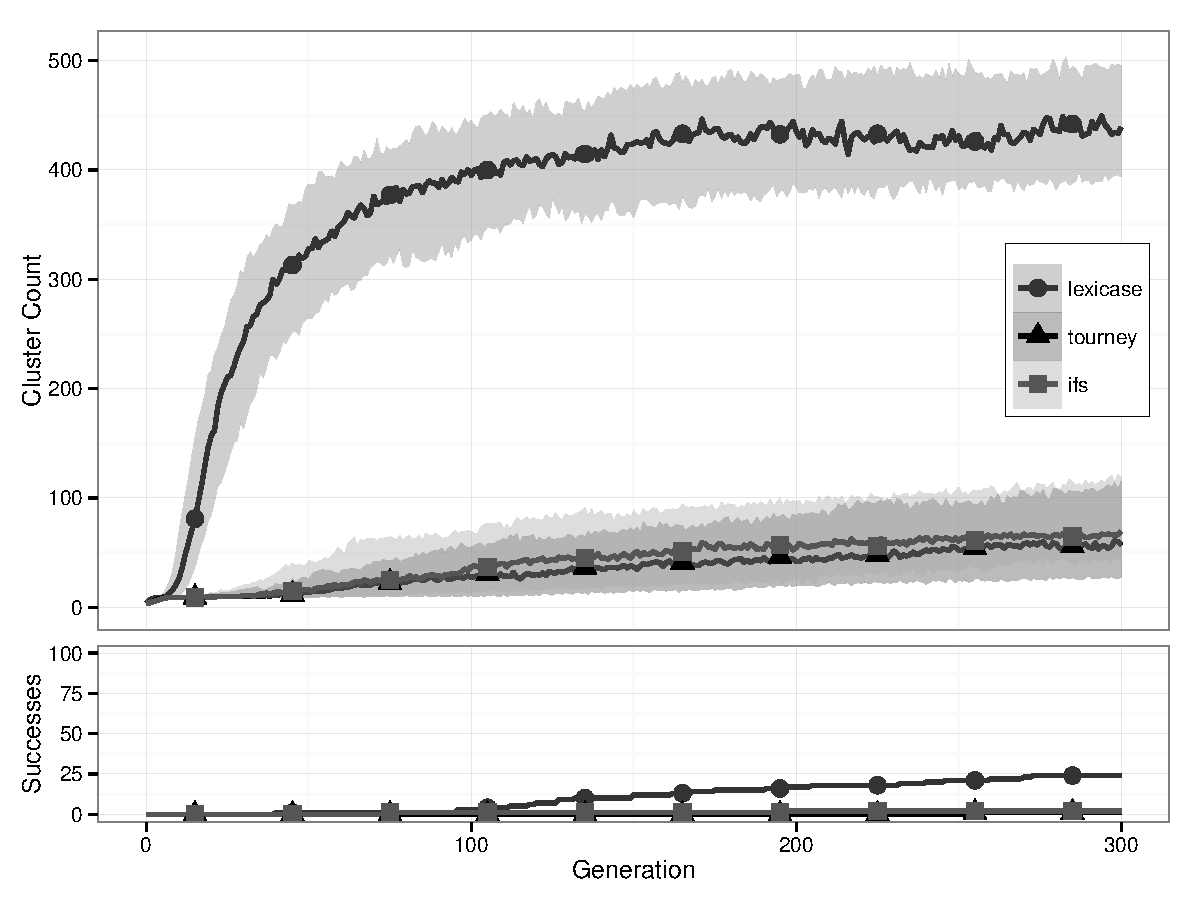
\includegraphics[width=11.5cm]{syllables-cluster.pdf}
\caption{Syllables -- cluster counts}
\label{syllablesClu}
\end{figure}

\begin{figure}[p] %[t] sets the image at the top of the page; t = top, b = bottom, h = here%
%\sidecaption[t]
\centering
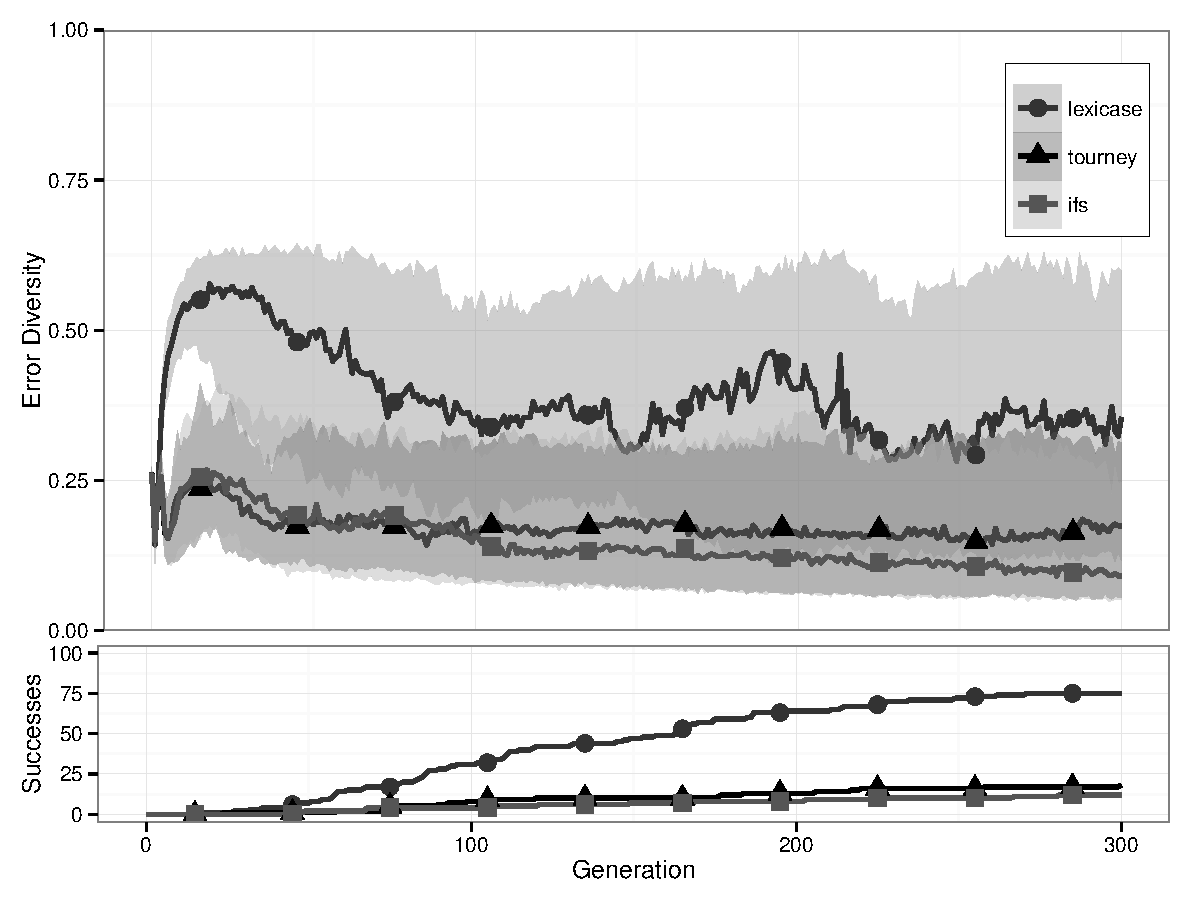
\includegraphics[width=11.5cm]{string-lengths-backwards-diversity.pdf}
\caption{String Lengths Backwards -- error diversity}
\label{string-lengths-backwardsDiv}
\end{figure}

\begin{figure}[p] %[t] sets the image at the top of the page; t = top, b = bottom, h = here%
%\sidecaption[t]
\centering
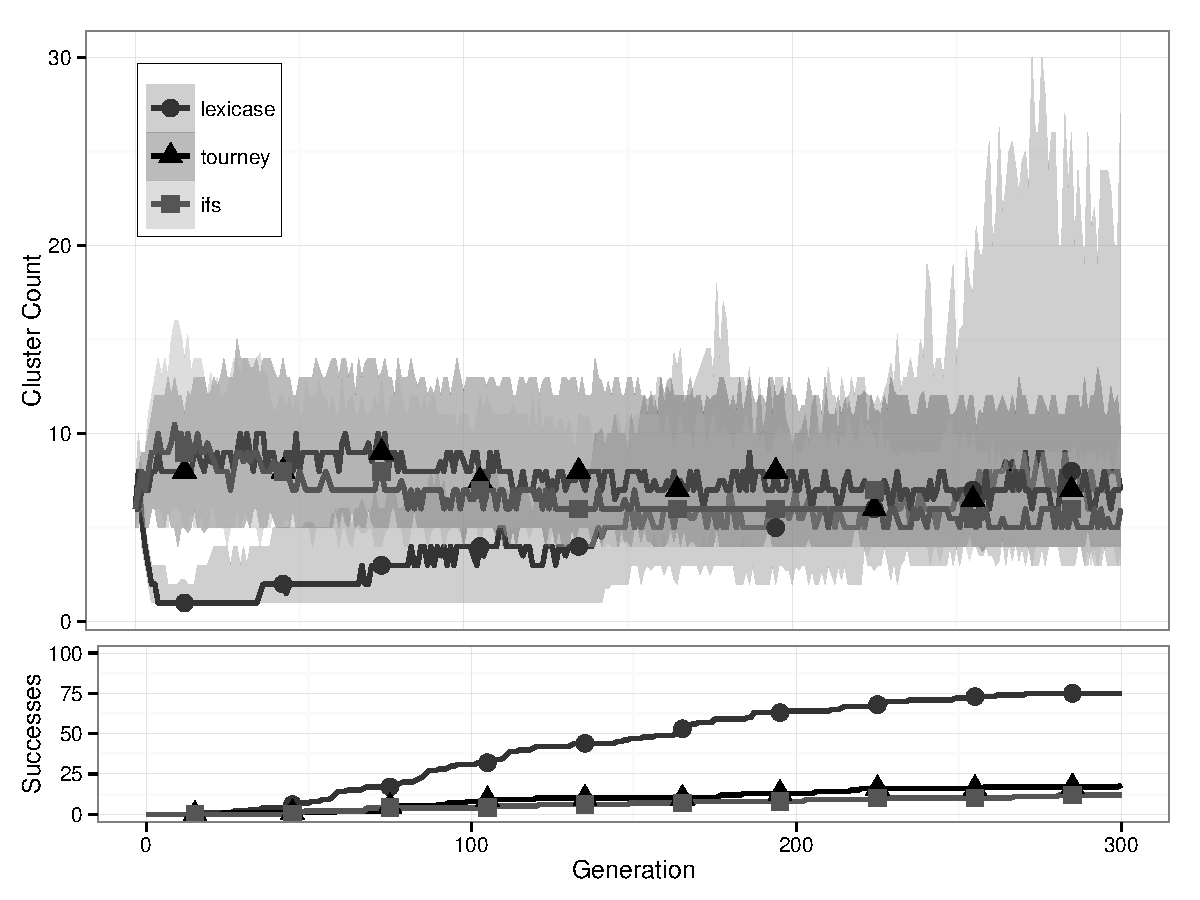
\includegraphics[width=11.5cm]{string-lengths-backwards-cluster.pdf}
\caption{String Lengths Backwards -- cluster counts}
\label{string-lengths-backwardsClu}
\end{figure}

\begin{figure}[p] %[t] sets the image at the top of the page; t = top, b = bottom, h = here%
%\sidecaption[t]
\centering
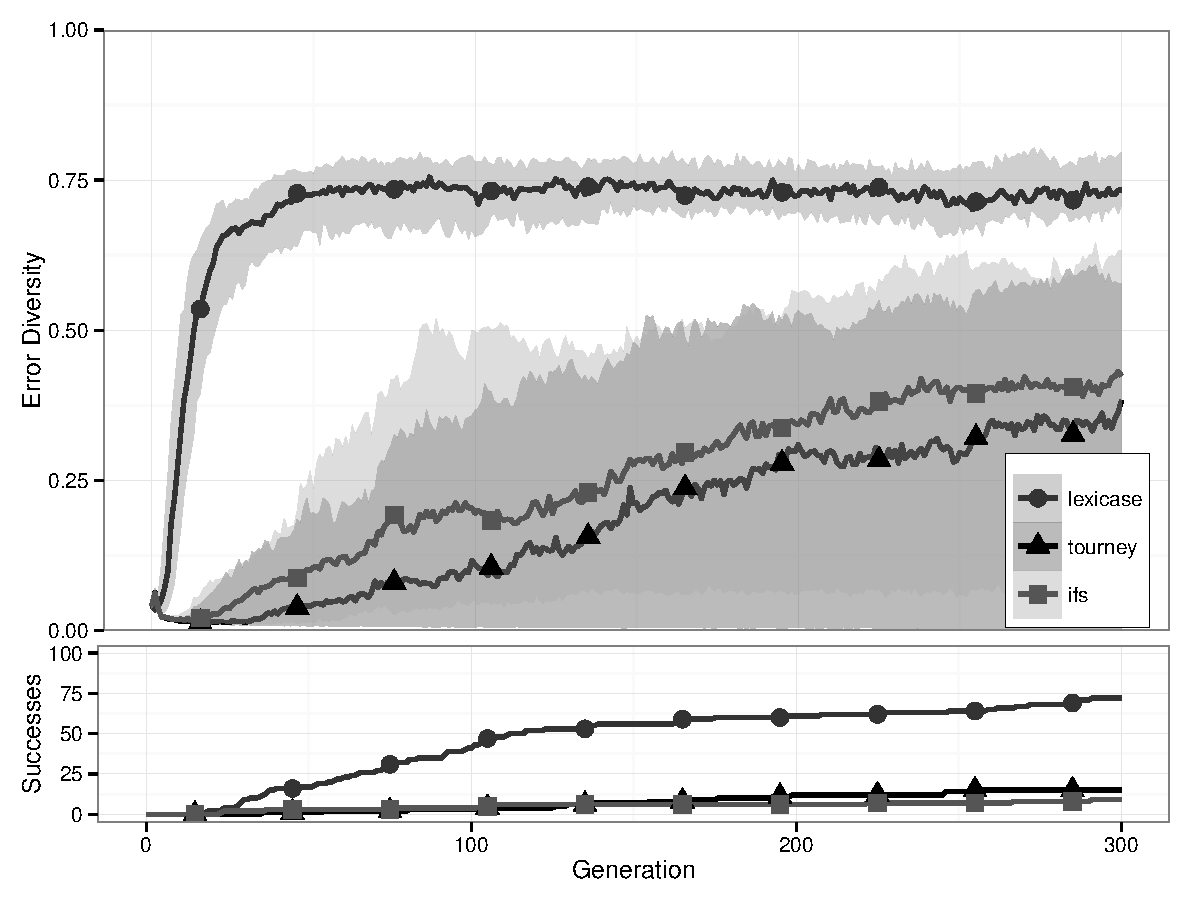
\includegraphics[width=11.5cm]{negative-to-zero-diversity.pdf}
\caption{Negative To Zero -- error diversity}
\label{negative-to-zeroDiv}
\end{figure}

\begin{figure}[p] %[t] sets the image at the top of the page; t = top, b = bottom, h = here%
%\sidecaption[t]
\centering
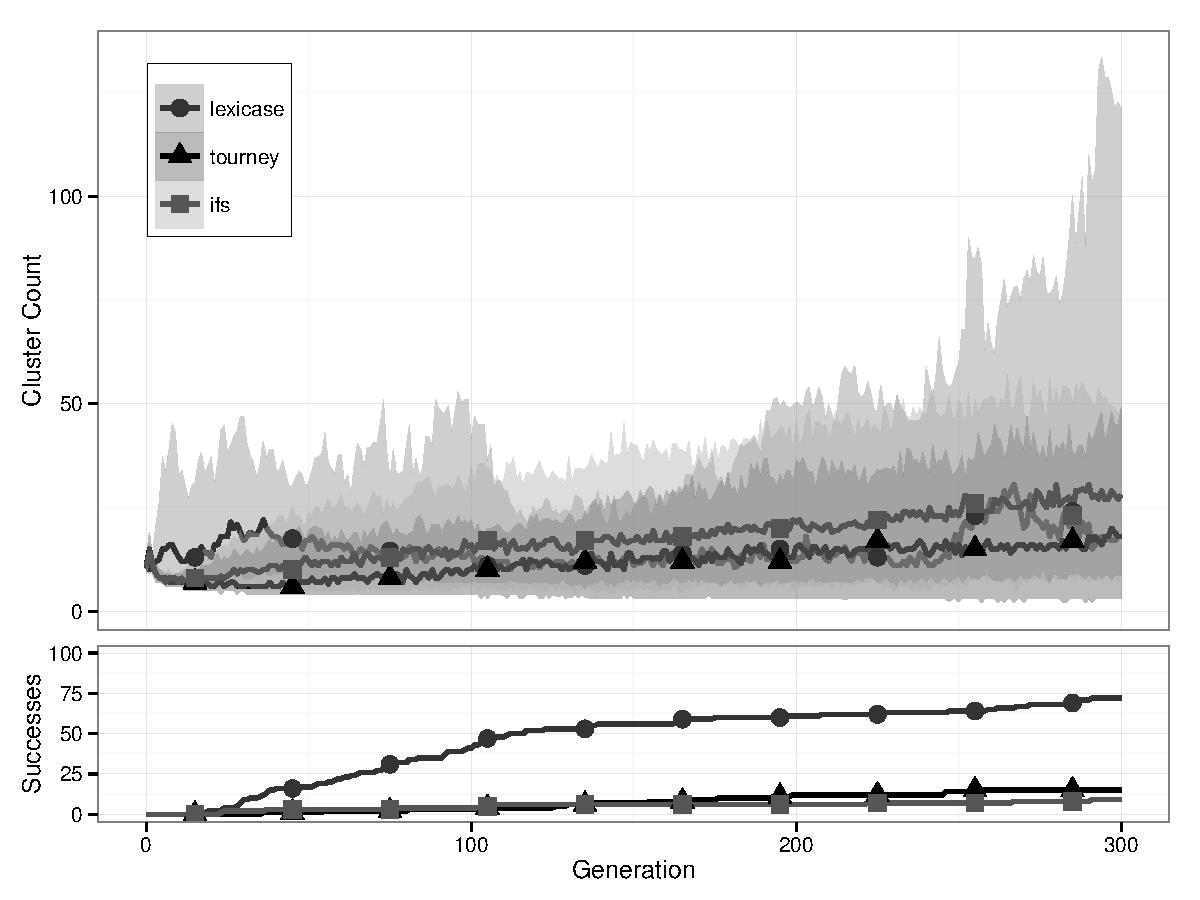
\includegraphics[width=11.5cm]{negative-to-zero-cluster.pdf}
\caption{Negative To Zero -- cluster counts}
\label{negative-to-zeroClu}
\end{figure}

\begin{figure}[p] %[t] sets the image at the top of the page; t = top, b = bottom, h = here%
%\sidecaption[t]
\centering
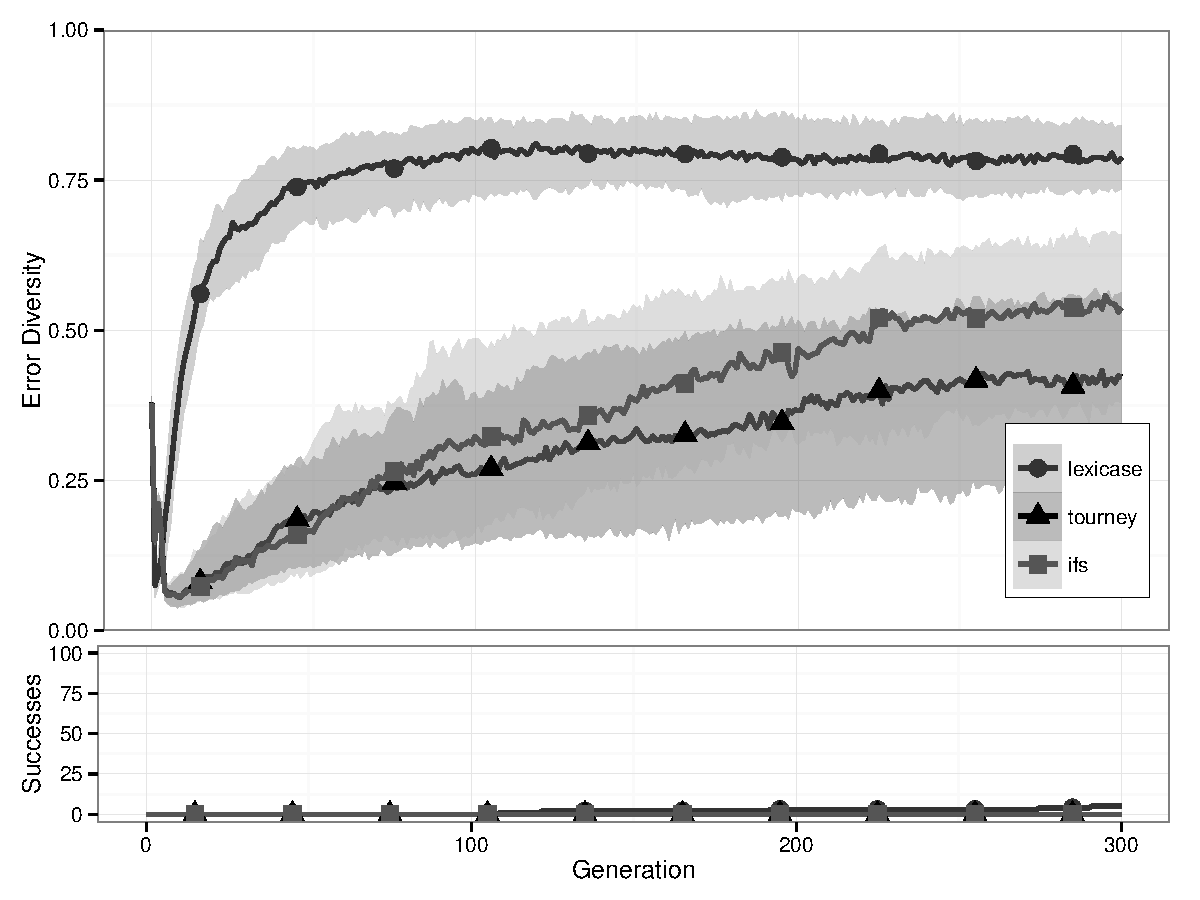
\includegraphics[width=11.5cm]{double-letters-diversity.pdf}
\caption{Double Letters -- error diversity}
\label{double-lettersDiv}
\end{figure}

\begin{figure}[p] %[t] sets the image at the top of the page; t = top, b = bottom, h = here%
%\sidecaption[t]
\centering
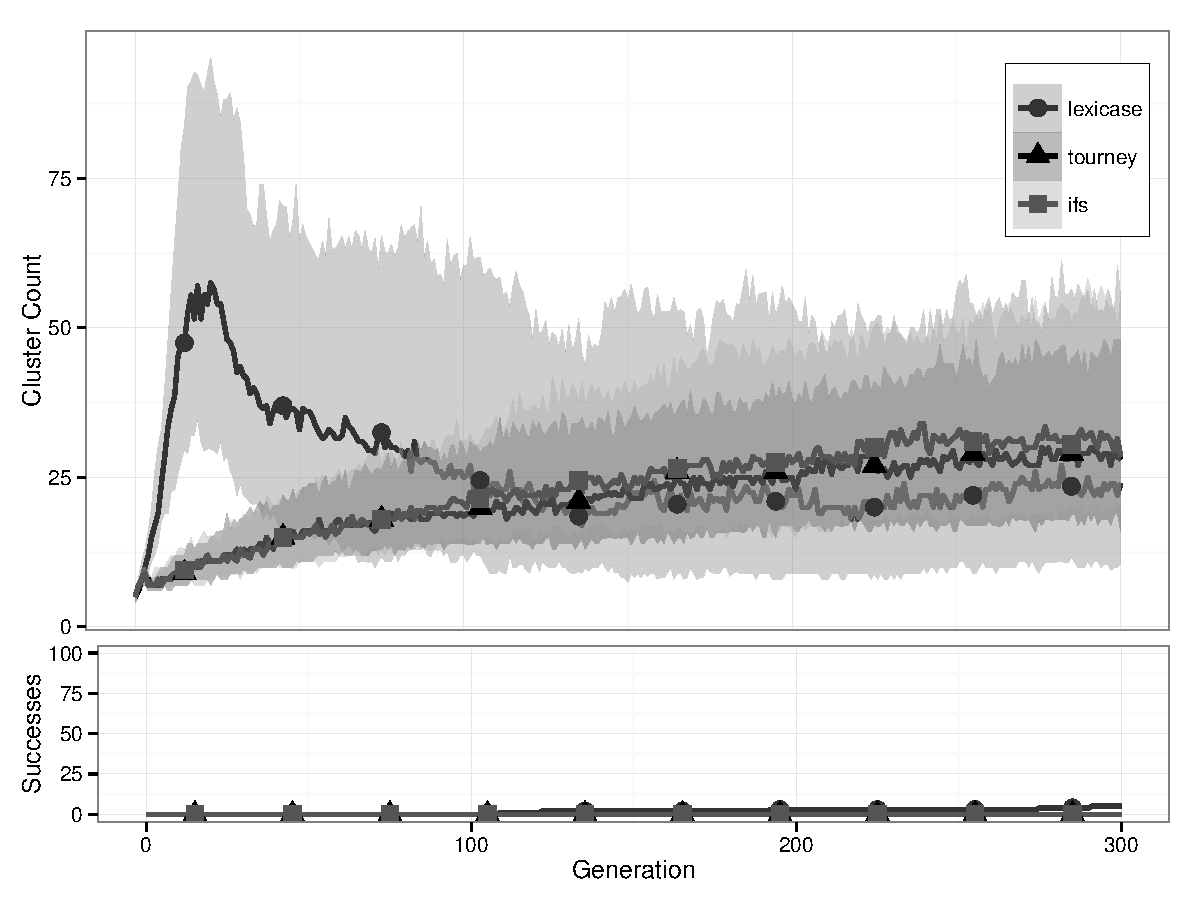
\includegraphics[width=11.5cm]{double-letters-cluster.pdf}
\caption{Double Letters -- cluster counts}
\label{double-lettersClu}
\end{figure}

\begin{figure}[p] %[t] sets the image at the top of the page; t = top, b = bottom, h = here%
%\sidecaption[t]
\centering
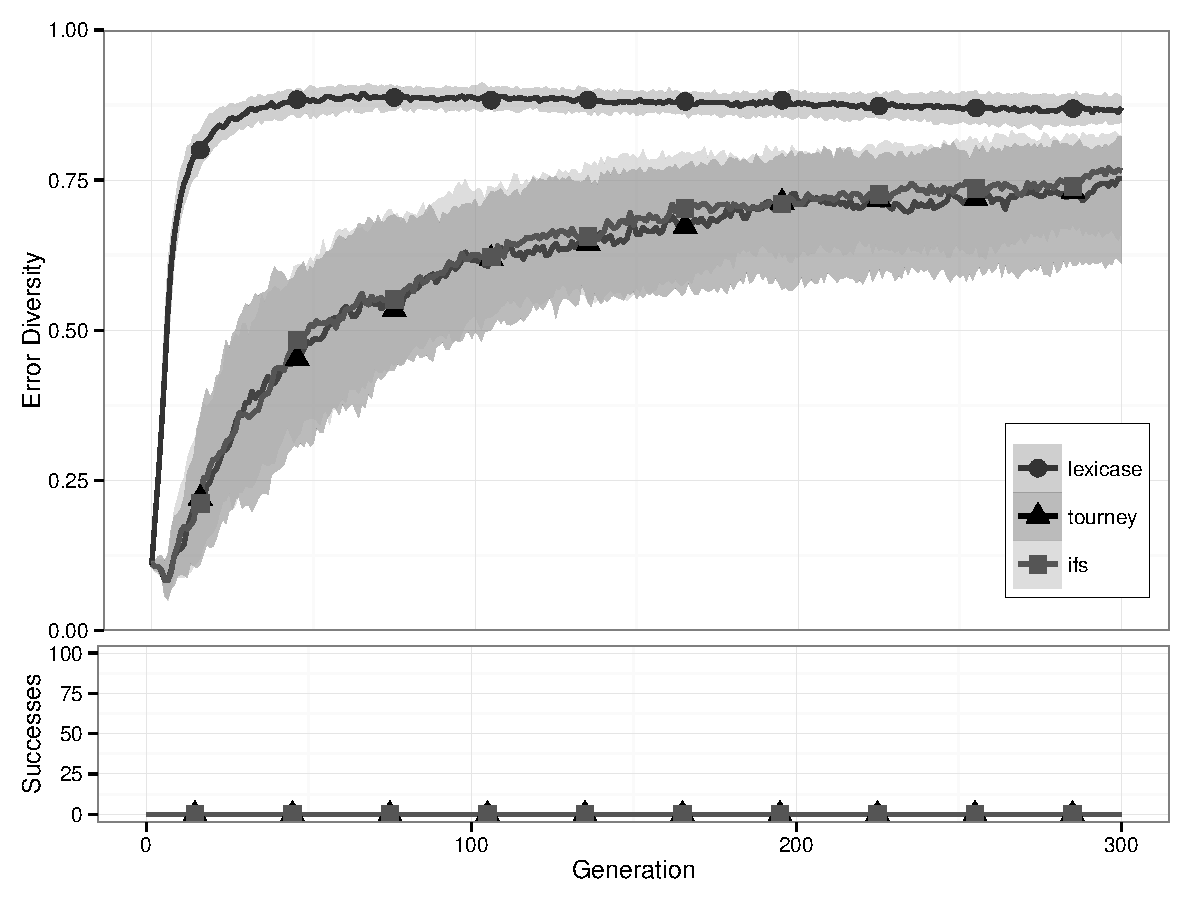
\includegraphics[width=11.5cm]{scrabble-score-diversity.pdf}
\caption{Scrabble Score -- error diversity}
\label{scrabble-scoreDiv}
\end{figure}

\begin{figure}[p] %[t] sets the image at the top of the page; t = top, b = bottom, h = here%
%\sidecaption[t]
\centering
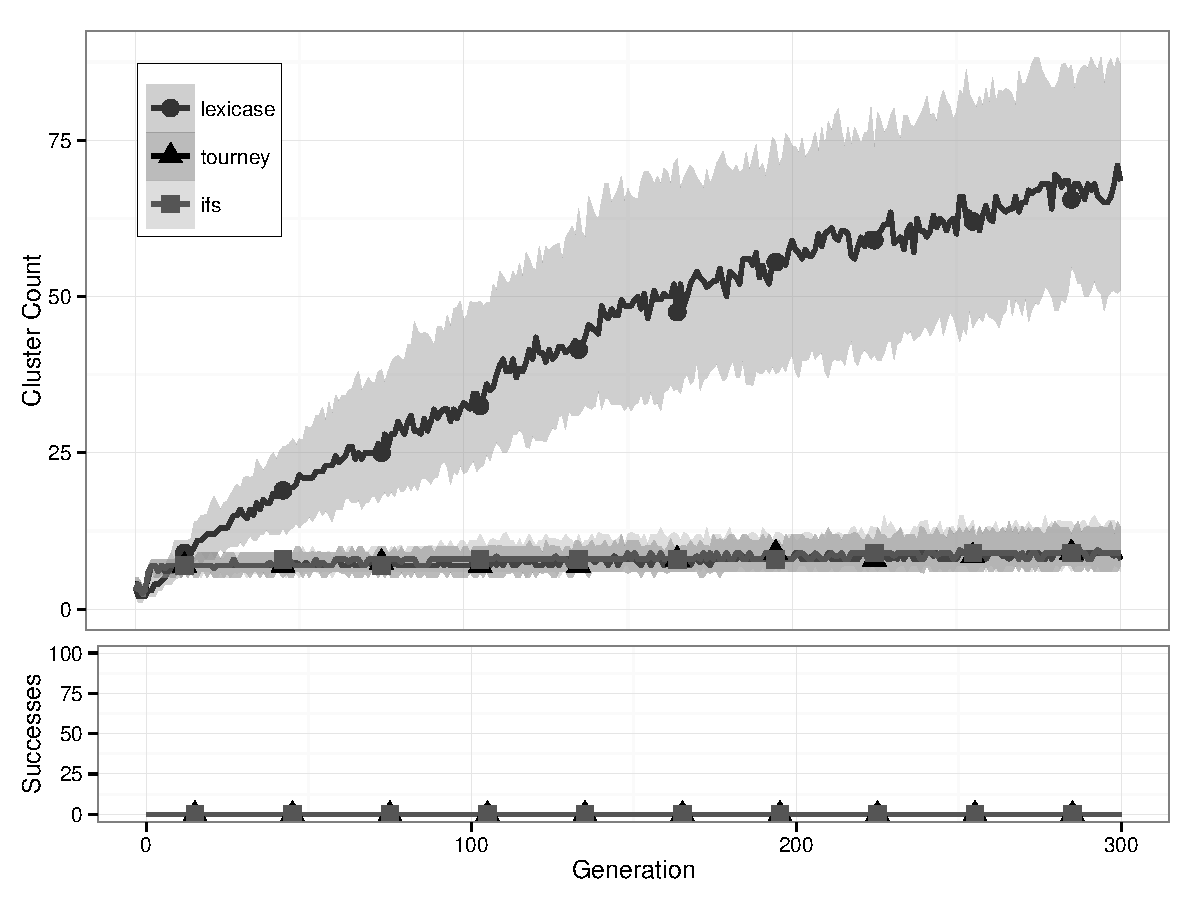
\includegraphics[width=11.5cm]{scrabble-score-cluster.pdf}
\caption{Scrabble Score -- cluster counts}
\label{scrabble-scoreClu}
\end{figure}

\begin{figure}[p] %[t] sets the image at the top of the page; t = top, b = bottom, h = here%
%\sidecaption[t]
\centering
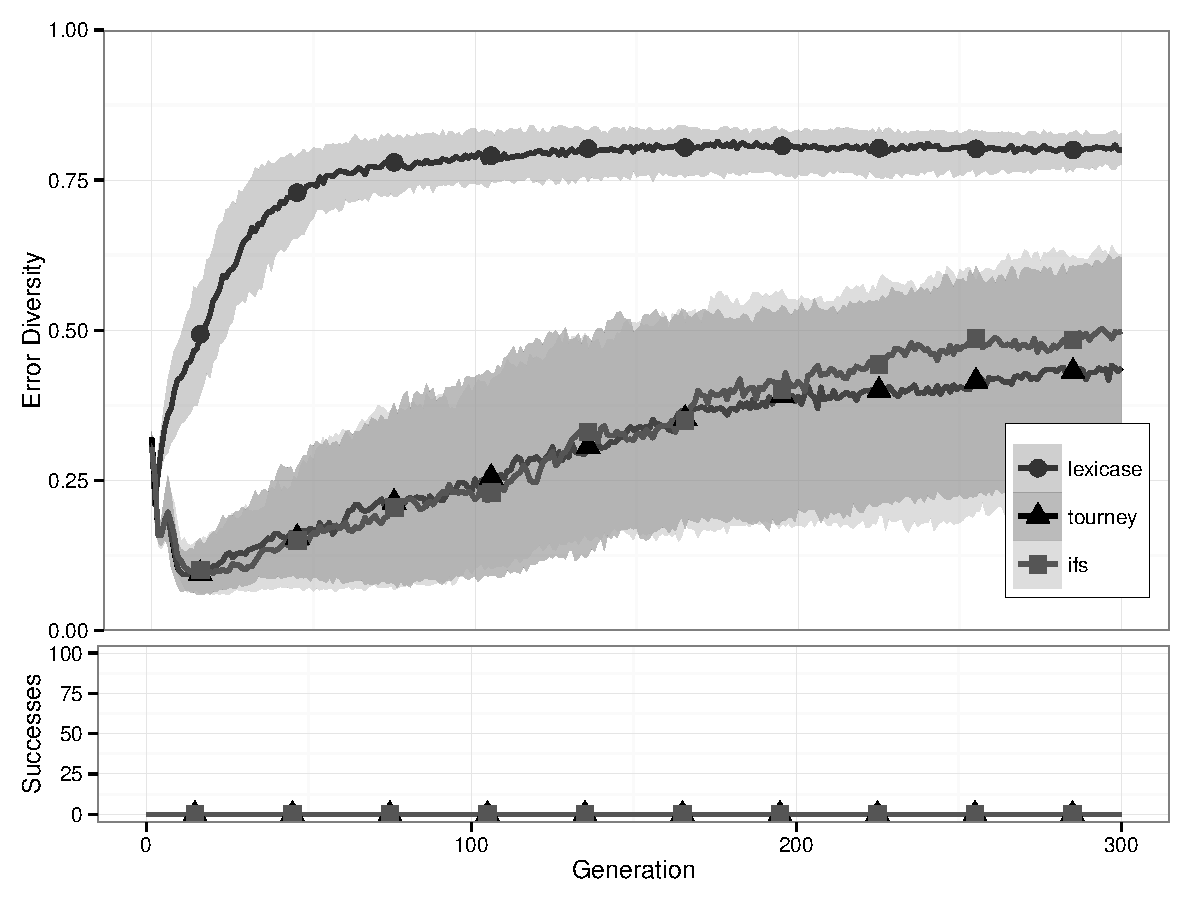
\includegraphics[width=11.5cm]{checksum-diversity.pdf}
\caption{Checksum -- error diversity}
\label{checksumDiv}
\end{figure}

\begin{figure}[p] %[t] sets the image at the top of the page; t = top, b = bottom, h = here%
%\sidecaption[t]
\centering
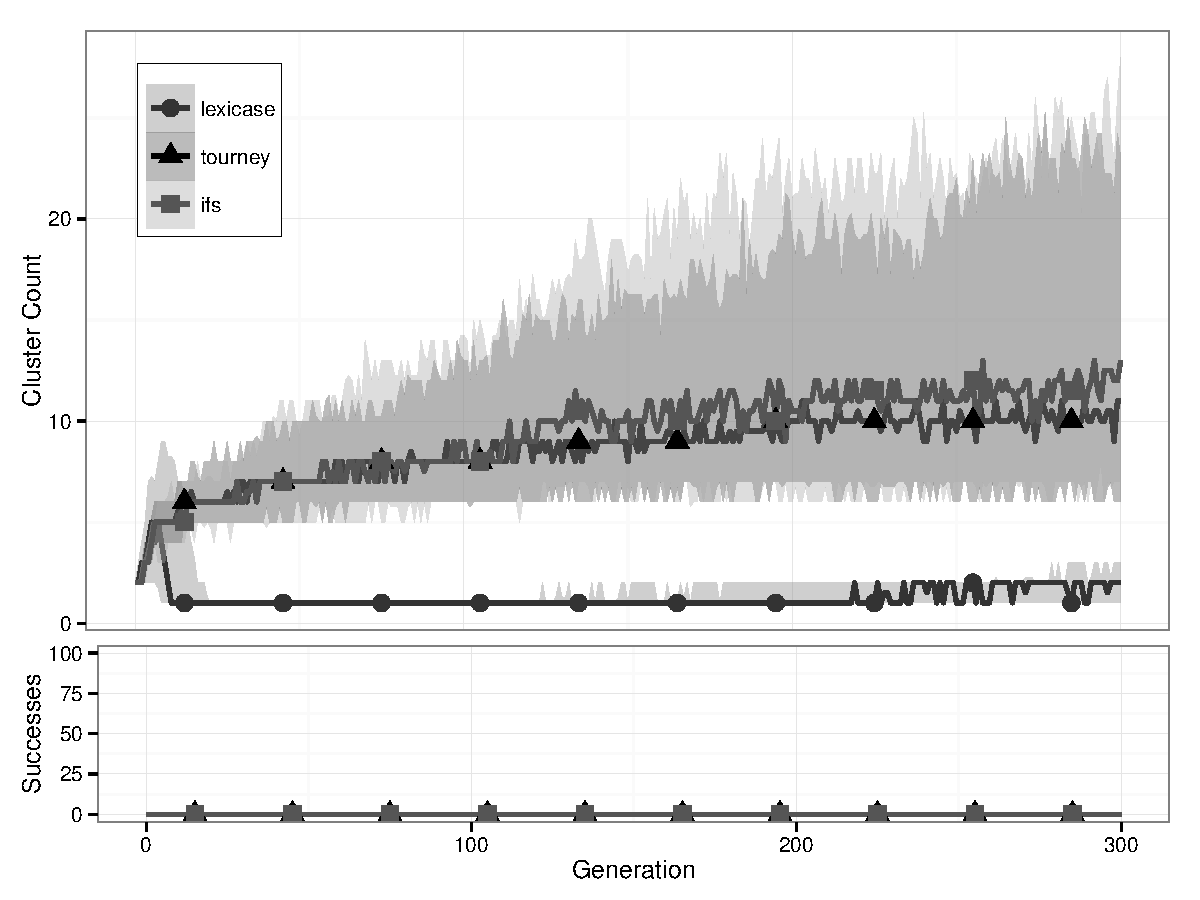
\includegraphics[width=11.5cm]{checksum-cluster.pdf}
\caption{Checksum -- cluster counts}
\label{checksumClu}
\end{figure}

\begin{figure}[p] %[t] sets the image at the top of the page; t = top, b = bottom, h = here%
%\sidecaption[t]
\centering
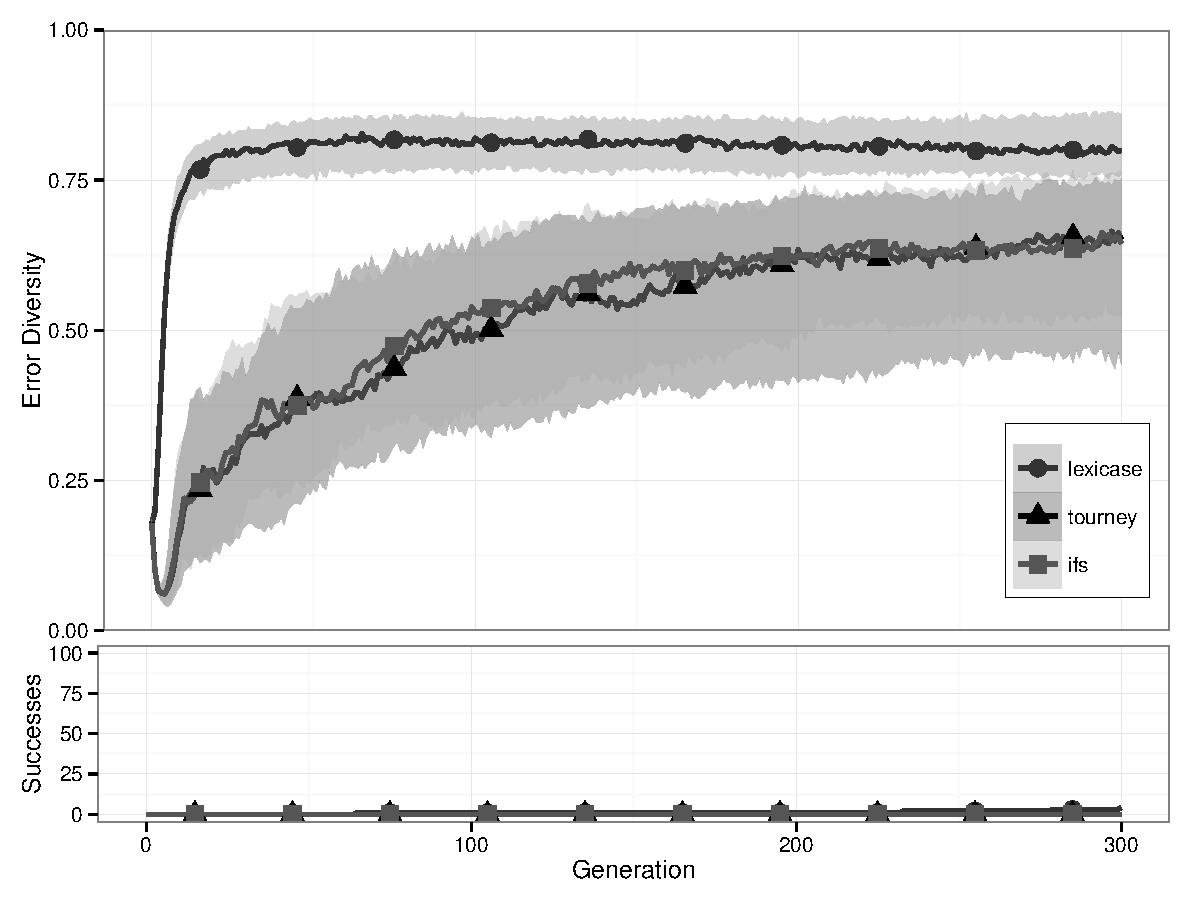
\includegraphics[width=11.5cm]{count-odds-diversity.pdf}
\caption{Count Odds -- error diversity}
\label{count-oddsDiv}
\end{figure}

\begin{figure}[p] %[t] sets the image at the top of the page; t = top, b = bottom, h = here%
%\sidecaption[t]
\centering
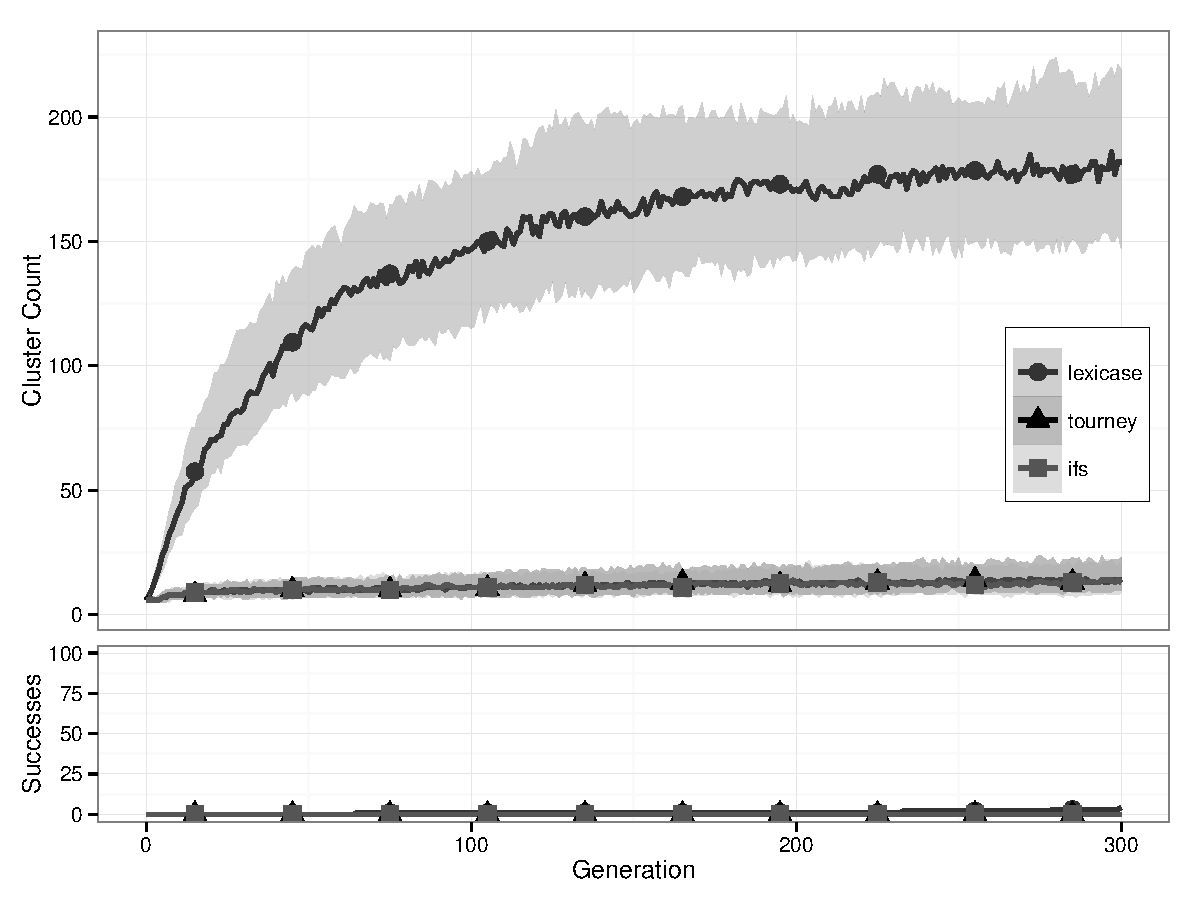
\includegraphics[width=11.5cm]{count-odds-cluster.pdf}
\caption{Count Odds -- cluster counts}
\label{count-oddsClu}
\end{figure}


\section{Discussion and importance of findings}
\label{sec:discussion}

As was the case in \cite{Helmuth:2015:GECCO}, lexicase selection had more successes than 
either tournament selection or IFS on any problem where a solution was discovered; no solution
was found for Scrabble Score or Checksum with this set of runs using any of the tested 
selection mechanisms. The error diversity for the lexicase runs was much higher than for tournament
selection and IFS for almost all eight problems, which is consistent with the hypothesis that
lexicase helps maintain diversity throughout the run. The lexicase error diversity values tended to
plateau at or above 0.75, meaning that in a population of 1,000 individuals there were over 700
\emph{distinct} error vectors. This doesn't ensure that different individuals were \emph{solving}
different test cases; it could just be that many individuals had slightly different incorrect
answers and error values for a few of the test cases. From a search perspective, though, this seems
preferable to having numerous individuals with the same error values, as hopefully those different
error values represent different starting points for subsequent search.

As mentioned in Section~\ref{sec:results}, for four of the eight problems, the cluster counts were
also much higher for lexicase than for the other two selection mechanisms. For some of these problems
(e.g., Count Odds) there are over 100 clusters, and for Syllables the median cluster count is over 400
from generation 100 forward. This means that there are hundreds of groups of individuals in these runs
whose error vectors are not just distinct, but that their elitized values differ on at least 10\%
of the test cases. For Count Odds, which has 200 test cases, that means there are consistently over
100 clusters, where each pair of clusters has different elitized values for at least 20 test cases.
This suggests that lexicase is maintaining large numbers of sub-groups of the population that are 
capable of solving different parts of the problem. If solutions aren't being discovered (and they're
not coming quickly) that might indicate that the genetic operators aren't able to act on the structure 
of the programs in those sub-populations in ways that allow progress.

Interpretation of the cluster count results on the other four problems is more difficult. Analysis
of some of the lexicase Checksum problem runs suggests that the lack of clustering might be a function
of some structural issues with the test cases.
For that problem there are 100 test cases, with two error functions per test case: the first uses Levenshtein edit distance on the printed string, and the second compares the last character of the printed string to the correct checksum character.
Looking at run
results, it appears that populations quickly evolve the ability to print \texttt{Check sum is}, but
then stall, with each program essentially producing a different set of random answers to the question
of what the checksum actually is. This allows for fairly high error diversity (over 0.75). This, however,
generates only one or two clusters as any given program tends to only get at most two or three test 
cases right by guessing, meaning that the manhattan distance between any two elitized error vectors
is typically only 5 or 6 at most, putting it well below the 10\% threshold of 20 in this case. This
suggests that a new set of test cases might improve the likelihood of success for Checksum, with
less emphasis on the fairly simple task of printing \texttt{Check sum is} and more single character
input strings, creating a broad group of test cases that only require the basic checksum calculation
on a single character and hopefully providing an initial gradient that evolution can use to gain
traction on the problem.

It is also worth noting that on problems where solutions were discovered, lexicase runs found solutions throughout the 300 generations. This, combined with the high levels of error diversity and the often 
high number of clusters gives one hope that meaningful search was in fact still happening, and that 
those runs were not hopelessly stalled. The plots of successes over time under the primary plots
typically appear to still have positive slope at generation 300, so it would be interesting to
extend these runs to 500 or 1,000 generations and see how many additional solutions are discovered.
If lexicase is indeed maintaining a meaningful pool of diversity, we would expect to see solutions continue
to be discovered, and at a higher rate than for either tournament selection or IFS. This might be
particularly interesting for problems where solution discovery is rare but possible, such as
Double Letters and Count Odds, which are solved using lexicase 5 and 3 times respectively, but not
at all using tournament selection and IFS. Solutions for these two problems tended to be discovered
later in the run (Double Letters in generations 109, 122, 192, 275, and 291; Count Odds in 65, 233, 279), so letting
runs on those problems go longer might be revealing.

On the set of problems explored here, error diversity seems to be a better predictor of performance than cluster counts. In fact, on two of the problems on which lexicase found solutions in over half the runs (String Lengths Backwards and Negative To Zero), lexicase maintained very small numbers of clusters, similar to tournament and IFS. On problems for which lexicase displayed many more clusters than the other methods (Syllables, Scrabble Score, and Count Odds), it found many fewer solutions. On the other hand, lexicase consistently maintained higher diversity than other methods, and found more solutions on every problem that was solved. This may indicate that the ability to form clusters on a problem is more indicative of the problem itself than the parent selection method and its ability to solve the problem. This provides evidence against our hypothesis that lexicase performs better because it maintains clusters of individuals that genetic operators combine to solve increasingly large numbers of test cases.

(TO DO: Nic: Tournament and IFS seem to be super similar. What, if anything, do we say about that?) (Tom: Firstly, this isn't too surprising when you consider that IFS is using tournaments. Thus, it is like it rearranges the rankings of the individuals, but then uses similar selection probabilities. It might be difficult to achieve more diversity with this selection probability mass function. The other thing to remark upon is that while IFS was devised as a diversity increaser, it doesn't seem to work that way in this setting. This indicates that it hasn't been sufficiently tested for diversity maintenance, at least for this type of problem. In places where it does increase performance, maybe it isn't because of diversity? Anyway, I'm not sure if we know what exactly to say here or if we'll have the room.)

\section{Conclusions}

In this paper we used two different measures of diversity (error diversity and cluster counts) to try to better understand the impact of Lexicase selection, and why it seems to consistently outperform tournament selection and implicit fitness sharing (IFS) on a range of software synthesis problems \cite{Helmuth:2015:GECCO}. The error diversity was generally \emph{much} higher for lexicase than with either tournament selection or IFS, showing that lexicase was able to maintain a broad range of distinct behaviors over the course of runs. The clustering counts were typically higher with lexicase, and the instances where they weren't may say more about the problem or test case structure than about the selection mechanism. This suggests that error diversity is definitely a valuable metric when trying to understand the impact of system design decisions on population diversity. The value of cluster counts is less clear, but it seems likely that understanding why the cluster counts were so low on certain problems could be informative.

Given that the Lexicase runs maintain error diversity all across the 300 generations, it seems plausible that extending the length of the runs would generate additional solutions; lexicase might still be effectively searching instead of hopelessly stalled due to convergence on some local optima. It would be illuminating to extend these runs to 500 or 1,000 generations and see whether lexicase is able to make ``better'' use of those additional computational resources.

While the focus of this paper was to better understand the behavior of lexicase selection, the results also show that for both diversty measures used here tournament selection and IFS seem to have \emph{very} similar behaviors, which seems unfortunate given that IFS was specifically designed to help maintain diversity. It's unclear why the IFS diversity figures weren't higher, but both are aggregating all their test case errors into a single value, with IFS just weighting the components differently. It would be worth exploring this further, but this might provide additional evidence for the importance in lexicase of not aggregating the test case errors into a single value.

\begin{acknowledgement}
	Thanks to the members of the Hampshire College Computational Intelligence Lab for discussions that helped to improve the work described in this paper, to Josiah Erikson for systems support, and to Hampshire College for support for the Hampshire College Institute for Computational Intelligence. This material is based upon work supported by the National Science Foundation under Grants No. 1017817, 1129139, and 1331283. Any opinions, findings, and conclusions or recommendations expressed in this publication are those of the authors and do not necessarily reflect the views of the National Science Foundation.
\end{acknowledgement}

\bibliographystyle{spbasic}
\bibliography{gp-bibliography,spector}
